\subsection{Rückenmark}
\label{subsec:Rueckenmark} \index{Rückenmark}
%%%%%%%%%%%%%%%%%%%%%%%%%%%%%%%%%%%%%%%%%%%%%%%%%%%%%%%%%%%
%%%%%%%%%%%%%%%%%%%%%%%%%%%%%%%%%%%%%%%%%%%%%%%%%%%%%%%%%%%

Das Rückenmark zeigt eine dorso-ventrale Organisation auf (Abb.~\ref{fig:ruckenmark_schema}). Dabei weist die zentral gelegene \textbf{graue Substanz}\index{graue Substanz}, die den Zentralkanal umgibt und die Somata der vorliegenden Neurone enthält, eine typische Schmetterlingsform auf. Generell kann zwischen dem Vorder- und Hinterhorn des Rückenmarks unterschieden werden. Im ventralen Vorderhorn (Grundplatte) sind die Somata der motorischen Fasern lokalisiert. Dabei sind die somatomotorischen Neurone eher ventral, die visceromotorischen eher dorso-lateral gelegen. Im dorsalen Hinterhorn (Flügelplatte), in dem die Somata der sensorischen Neurone liegen, sind die somatosensorischen Neurone eher dorsal gelegen, die viscerosensorischen eher ventral.\\

\noindent Die \textbf{weiße Substanz}\index{weiße Substanz} umgibt peripher die graue Substanz. Sie enthält neben Gliazellen und Blutgefäßen ausschließlich markhaltige Fasern. Dabei verlaufen sowohl die aufsteigenden, als auch die absteigenden Bahnen in der weißen Substanz. Des Weiteren treten pro Körpersegment jeweils zwei laterale Nerven aus, die \textbf{dorsale und ventrale Wurzel} genannt werden (Abb.~\ref{fig:ruckenmark_schema}). Diese vereinen sich in kurzem Abstand zum Rückenmark zu \textbf{Spinalnerven}. Kurz vor dieser Vereinigung von dorsaler und ventraler Wurzel ist eine Schwellung erkennbar, das sogenannte \textbf{Spinalganglion}. Dieses dient der metabolischen Versorgung, sowie der Energieversorgung der vorliegenden Neurone. Nach der Vereinigung zum Spinalnerv spaltet sich dieser erneut in drei Äste (Rami) auf (Abb.~\ref{fig:ruckenmark_wirbelsaeule}) \textsuperscript{\cite[Kap.~14]{penzlin2005tierphys}}.

\begin{figure}[H]
     \centering
     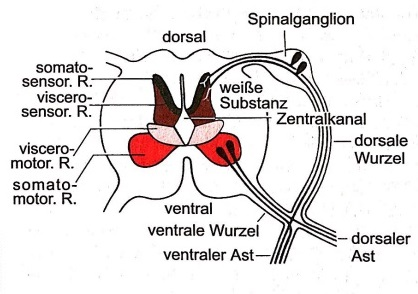
\includegraphics[width=0.59\textwidth]{pictures/Bilder_Jule/Andere/rueckenmark_schema.jpg}
     \caption[Aufbau des Rückenmarks]{\textbf{Aufbau des Rückenmarks.} Gezeigt ist ein schematischer Querschnitt durch das Rückenmark. Das dorsale Hinterhirn liegt oben, das ventrale Vorderhorn unten. Abbildung aus \textit{Lehrbuch der Tierphysiologie}, Penzlin \textsuperscript{\cite[Kap.~14]{penzlin2005tierphys}}.}
     \label{fig:ruckenmark_schema}
 \end{figure}{}

\noindent Innerhalb der Wirbelsäule ist das Rückenmark, wie auch das Gehirn innerhalb des Schädel-knochens, von mehreren Hüllen umgeben. Bei der innersten, ersten Schicht handelt es sich um die weiche \textbf{Pia mater}\index{Hirnhäute}. Zwischen der weichen Pia mater und der äußeren, festeren \textbf{Dura mater spinalis} befindet sich der \textbf{Subarachnoidalraum}, der mit Liquor gefüllt ist. Das Rückenmark ist an mehreren seitlichen Bändern, den \textbf{Ligamenta denticulatum}, im Subarachnoidalraum befestigt, bzw. aufgehängt (Abb.~\ref{fig:ruckenmark_wirbelsaeule}). 

\begin{figure}[H]
     \centering
     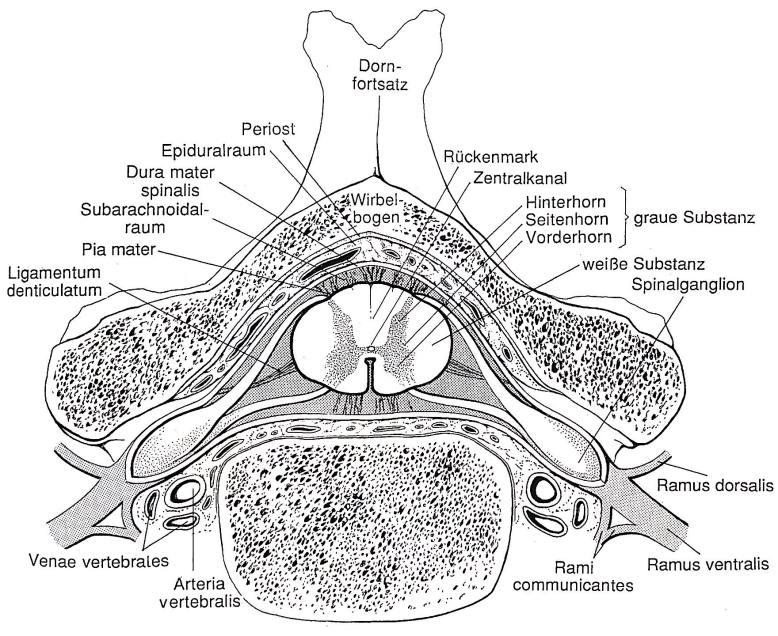
\includegraphics[width=0.79\textwidth]{pictures/Bilder_Jule/Andere/rueckenmark_wirbelsaeule.png}
     \caption[Querschnitt durch Wirbelsäule und Rückenmark]{\textbf{Querschnitt durch Wirbelsäule und Rückenmark.} Aufhängung des Rückenmarks innerhalb der Wirbelsäule eines höheren Primaten. Die dorsale Seite ist nach oben, die ventrale nach unten orientiert.\\
     Abbildung aus \textit{Kurzes Lehrbuch der Zoologie}, Storch und Welsch \textsuperscript{\cite[Kap.~6]{storch2012lehrbuchzoo}}.}
     \label{fig:ruckenmark_wirbelsaeule}
\end{figure}
